\def\difficulty{3}
\sujet{Geometry of Gaussian Random Fields}
\index{Random Fields}

\begin{note}This tutorial aims at simulating Gaussian random fields and analyzing their geometry.\end{note}

\section{Introduction}
Let $\phi$ be a real-valued stationary Gaussian Random Field (GRF) on $\R^2$. $\forall p\in\R^2$, $\phi(p)$ defines a random variable. The family $(\phi(p),p\in\R^2)$ consists of identically distributed random variables on a probability space $\Omega, \mathcal{F}, P$ that satisfies for any subset of $\{p_1,...,p_n \in \R^2\}$ and $\alpha_k\in\R$ that the random variable $\sum_{k=1}^n \alpha_k \phi(p_k)$ is normally distributed. The reader could find more informations in \cite{Worsley1997,Adler1981,Ahmad2013}.

Thus, $\phi$ is completely characterized by its mean and its covariance:
\begin{alignat}{4}
 m   \ =\ &\E(\phi(p)) &\ =\ & \E(\phi(0))                         &,\ & p\in\R^2 \\
 C(p)\ =\ &\E(\phi(0)\phi(p))-m^2 &\ =\ & \E(\phi(q)\phi(p+q))-m^2 &,\ & p,q \in \R^2
\end{alignat}

\textls[-15]{In this tutorial, we will assume $m\!=\!0$. The goal is to construct $\phi$ for a given covariance $C$.}

% \subsection*{Utility}
% For saving random fields into image files, you can use the following function:
% \begin{lstlisting}
% function I = imwrite_rf(R, name)
% % function that write a random field in a color image
% %
% % R: random field
% % name: name of the image
% %
% % I: color image rgb
% I = ind2rgb(uint8(R), jet(256));
% imwrite(I, name);
% \end{lstlisting}


\section{Simulation}
For more details on algorithms simulating GRFs in $\R^d$, see \cite{Lang2011}.

\subsection{Gaussian white noise random field}

\begin{qbox}
\begin{itemize}
 \item 
Generate a white noise on $\R^2$. Choose an $n\times n$ size. Display it on the screen (see for example Fig. \ref{fig:wn}).
\item 
Modify the variance and observe the results.
\end{itemize}
\end{qbox}

\begin{mcomment}
\begin{mremark}
 Use \minline{randn} and \minline{imagesc} or \minline{imshow}.
\end{mremark}
\end{mcomment}

\begin{pcomment}
\begin{premark}
 Use \pinline{randn} from \pinline{numpy.random}. Use \pinline{imshow} from \pinline{matplotlib.pyplot}.
\end{premark}
\end{pcomment}


\begin{figure}[H]
\centering\caption{Gaussian White Noise, with $m=128$ and $\sigma=30$ for display purposes.}%
 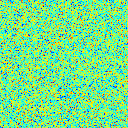
\includegraphics[width=4cm]{../matlab/wn.png}%
 \label{fig:wn}%
\end{figure}

\subsection{Gaussian Random Field}
Let $W$ be an independent centered white noise random fields. $\fft$ is the Fourier Transform. The gaussian random field $\phi$ is defined by:
$$p\in\R^2, \phi(p) = \fft^{-1}(\hat{\phi})(p)$$
and 
$$ \hat{\phi}(k) = \sqrt{\fft(C)(k)\fft(W)}$$


\begin{qbox}
\begin{itemize}
 \item Generate a 2D Gaussian covariance function , see Fig. \ref{fig:gaussienne} (we recall the definition, $u^2=x^2+y^2$):
 $$C(u)=e^{-\frac{u^2}{2\sigma^2}}$$
 

 \item Generate the Gaussian random field (see Fig. \ref{fig:grf}). Test with different values of $\sigma$.
\end{itemize}
\end{qbox}

\begin{mcomment}
\begin{mremark}
 Use \minline{meshgrid} for efficiency.
\end{mremark}
\end{mcomment}

\begin{pcomment}
\begin{premark}
 Use \pinline{meshgrid} from \pinline{numpy}.
\end{premark}
\end{pcomment}



\begin{figure}[H]
  \centering\caption{Covariance and Gaussian random field examples.}%
  \subfloat[Generation of a 2D Gaussian function.]{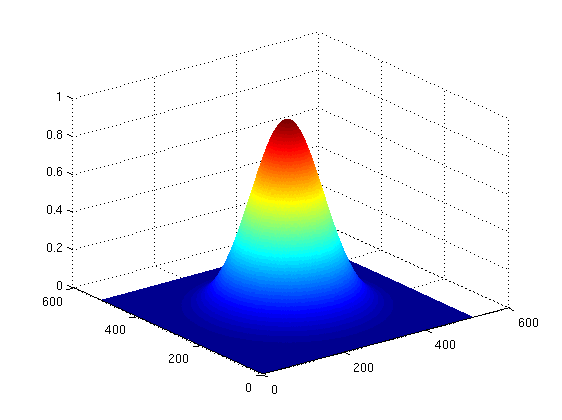
\includegraphics[width=.45\textwidth]{../matlab/gaussienne.png}\label{fig:gaussienne}}
 \hfill
  \subfloat[Generation of a 2D Gaussian random field with Gaussian covariance.]{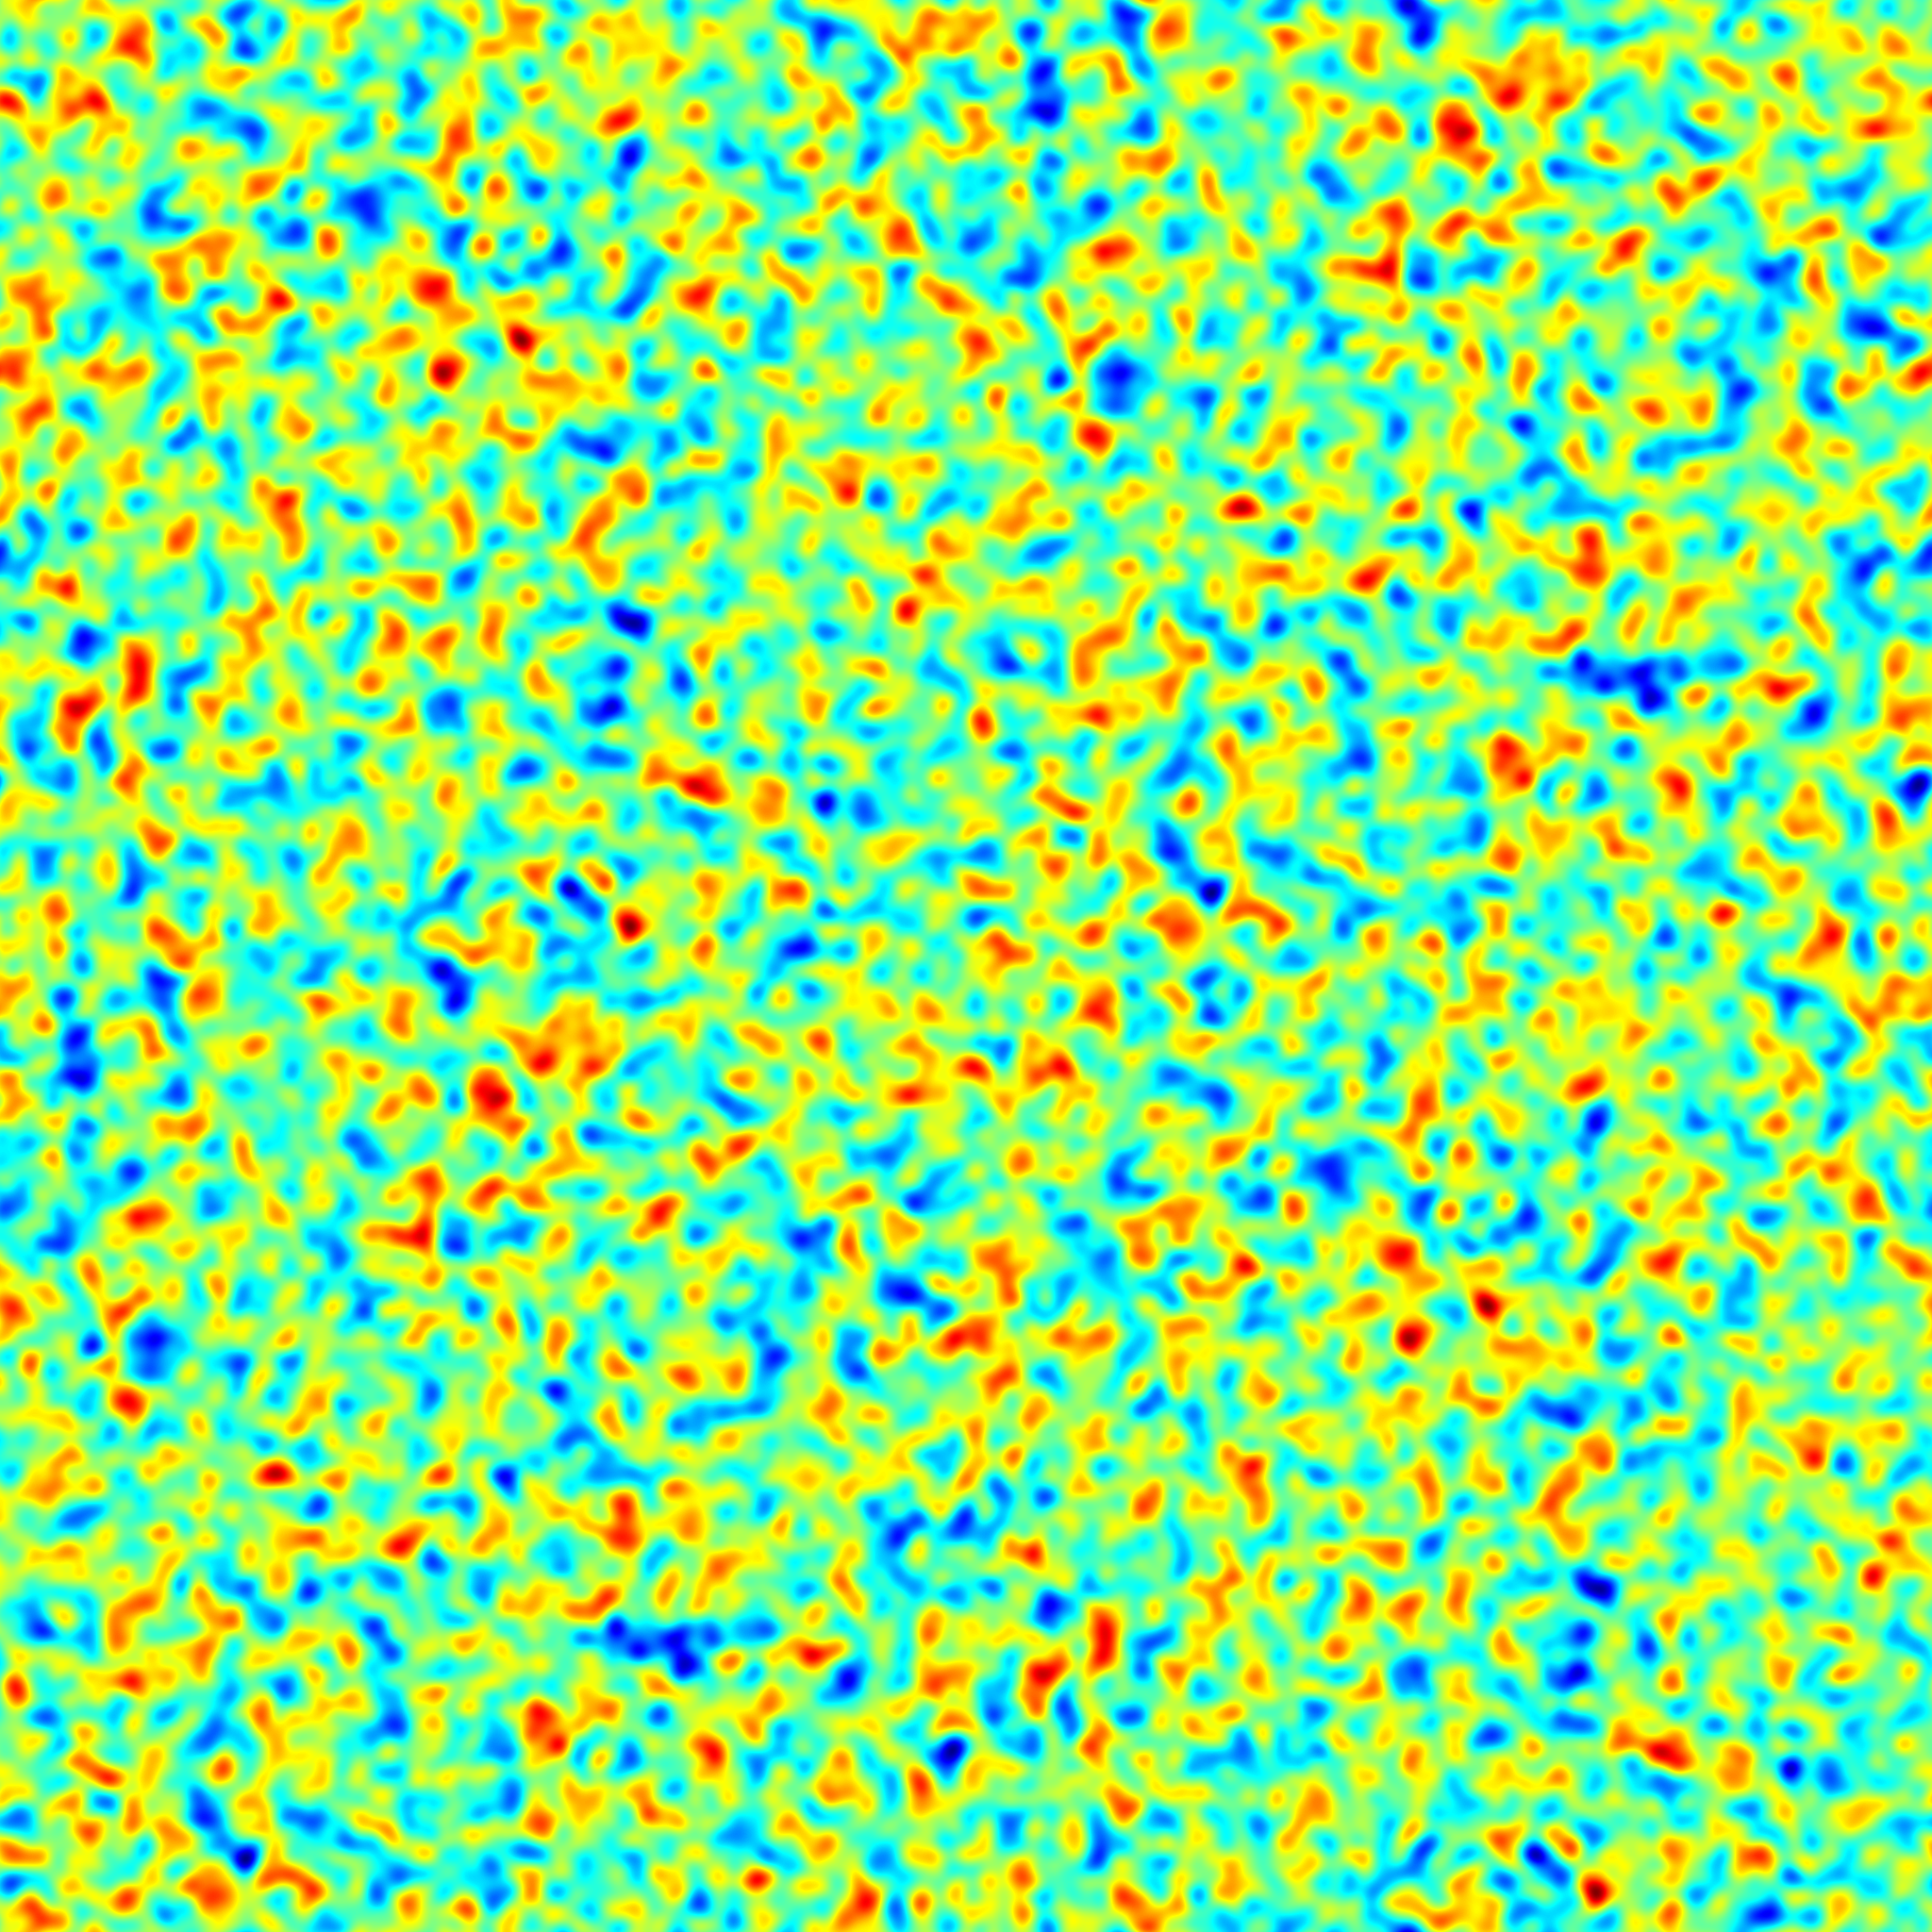
\includegraphics[width=.45\textwidth]{../matlab/grf.png}\label{fig:grf}}%
\end{figure}
\section{Geometry}
\subsection{Excursion set}
Let $Y(x)$, $x\in\R^2$, be a stationary real-valued random field. An excursion set, denoted by $E_h(Y, S)$, of $Y$ inside a compact subset $D\subset \R^2$ above a level $h$, is defined as:
$$E_h(Y,D) = \{ p\in D: Y(p)\geq h\}$$

In $D\subset\R^2$, an excursion set is a binary image.

\begin{qbox}
Represent, for each level $h$, the area $A$, the perimeter $P$ and the Euler number $\chi$ of $E_h(Y,D)$ (see Fig. \ref{fig:mf}). You can have a look at the tutorial \iflabelexists{
tutorial:integral_geometry:enonce}{\ref{tutorial:integral_geometry:enonce} }{about integral geometry} for perimeter, area and Euler number computation.
\end{qbox}

\begin{mcomment}
\begin{mremark}
\minline{bwperim(levelset)}, \minline{bwarea} and \minline{bweuler(levelset)} can be useful. Use default values for the neighborhood.
\end{mremark}
\end{mcomment}

\vspace*{-8pt}

 \begin{figure}[H]
   \centering\caption{Example of computation of Area, Perimeter and Euler number of level sets $E_h$.}%
   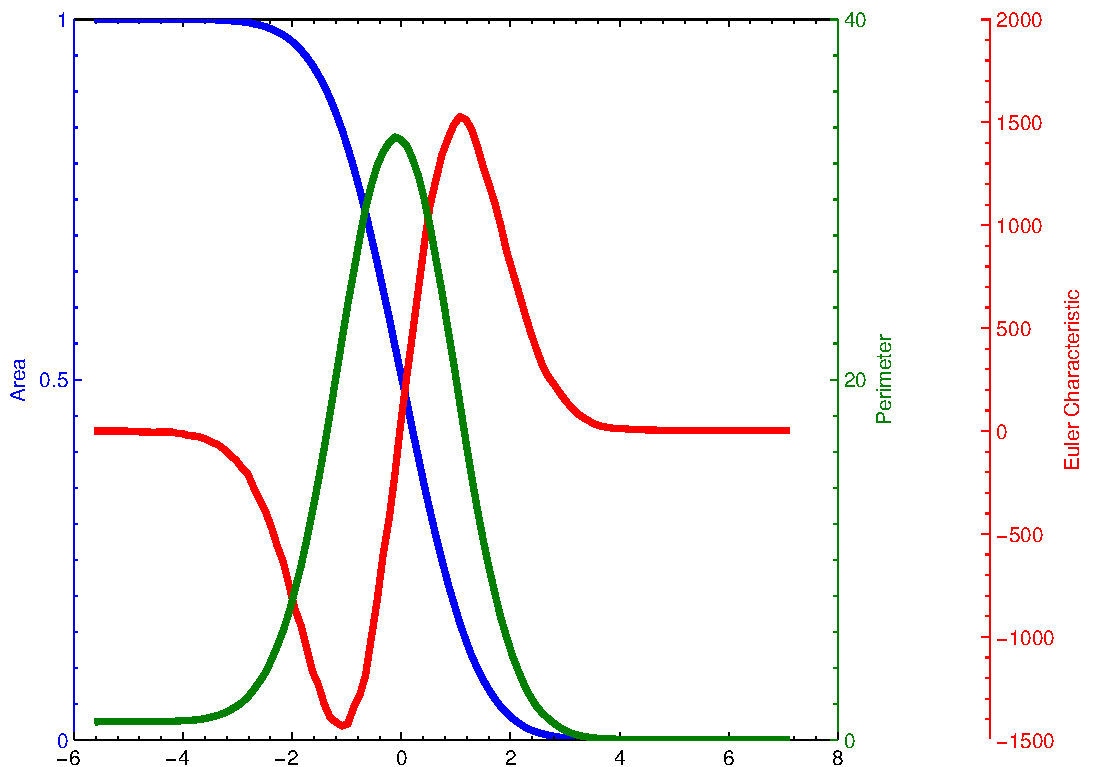
\includegraphics[width=7.8cm]{gaussian_t_rf_5.pdf}%
   \label{fig:mf}
  \end{figure}

\vspace*{-12pt}


\subsection{Analytical values}
We define three values, area $A$, perimeter $C$ (Contour length) and Euler number $\chi$, as functions of the level $h$, with:
\begin{eqnarray}
 A(h) &=& \mathcal{L}_2(D)\rho_0(h) \\
 C(h) &=& 2\left(\mathcal{L}_1(D)\rho_0(h) + \frac{\pi}{2}\mathcal{L}_2(D) \rho_1(h)\right)\\
 \chi(h) &=& \mathcal{L}_0(D)\rho_0(h) + \mathcal{L}_1(D)\rho_1(h)+\mathcal{L}_2(D) \rho_2(h)
\end{eqnarray}
with $\mathcal{L}_0(D)=\chi(D)=1$, $\mathcal{L}_1(D)$ is half the boundary length of the rectangle $D$ and $\mathcal{L}_2(D)$ is its area.

\begin{qbox}
\begin{itemize} \item First, compute the following values:
 \begin{align}
  \rho_0(h) &= \int_h^\infty \frac{1}{\sqrt{2\pi}} e^{-u^2/2}du \\
  \rho_1(h) &= \frac{\sqrt{\lambda}}{2\pi}e^{-h^2/2} \\
  \rho_2(h) &= \frac{\lambda}{(2\pi)^{\frac{2}{3}}}e^{-h^2/2}h \\
  \lambda &= \frac{1}{\sigma^2}
 \end{align}
 
 \item Then, compute the analytical values of $A$, $C$ and $\chi$.
 \item Compare the analytical values to the empirical ones.
 \end{itemize}
\end{qbox}

\begin{mcomment}
\begin{mremark}
Use \minline{erf}.
\end{mremark}
\end{mcomment}

\begin{pcomment}
\begin{premark}
Use \pinline{erfc} from \pinline{scipy.special}.
\end{premark}
\end{pcomment}

